\documentclass[border=3pt]{standalone}
\usepackage{tikz}
\usetikzlibrary{arrows.meta,calc,positioning}
\tikzset{pin/.style={-{Stealth[length=5pt]}},
  blk/.style={draw, thick, minimum width=18mm, minimum height=9mm, font=\sffamily\small, align=center}}
\begin{document}
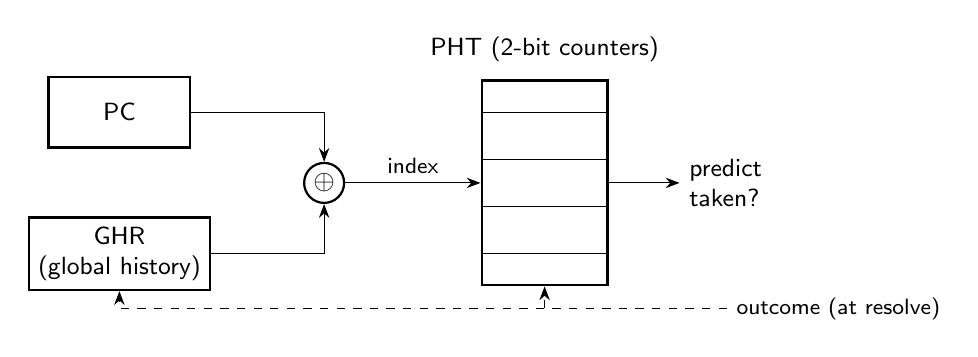
\begin{tikzpicture}[font=\sffamily\small]
  \node[blk] (pc)  at (0,0.9)  {PC};
  \node[blk] (ghr) at (0,-0.9) {GHR\\(global history)};
  % xor
  \node[draw, thick, circle, inner sep=1.5pt, font=\sffamily] (xor) at (2.6,0) {$\oplus$};
  \draw[pin] (pc.east)  -| (xor.north);
  \draw[pin] (ghr.east) -| (xor.south);
  % PHT table
  \node[draw, thick, minimum width=16mm, minimum height=26mm, font=\sffamily\small, align=center] (pht) at (5.4,0) {};
  \node[font=\sffamily\small, above=1mm of pht.north] {PHT (2-bit counters)};
  \foreach \y in {-9,-3,3,9}{\draw ($(pht.west)+(0,\y mm)$) -- ($(pht.east)+(0,\y mm)$);}
  \draw[pin] (xor.east) -- node[above, font=\sffamily\footnotesize]{index} (pht.west);
  % output
  \draw[pin] (pht.east) -- ++(9mm,0) node[right, font=\sffamily\small, align=left]{predict\\taken?};
  % update path
  \draw[pin, dashed] ($(pht.east)+(15mm,-16mm)$) node[right, font=\sffamily\footnotesize]{outcome (at resolve)} -| (pht.south);
  \draw[pin, dashed] ($(pht.east)+(15mm,-16mm)$) -| (ghr.south);
\end{tikzpicture}
\end{document}
